% !TeX root = ../document.tex

\chapter{施瓦西时空}

\begin{xiti}
	\item 考虑 Taub 的平面对称时空,其线元为式 (8-6-1')\footnote{正文(8-6-1')为
	\begin{equation*}
		\dd{s}^2 = z^{-1/2} \left( - \dd{t}^2 + \dd{z}^2 \right) + z \left( \dd{x}^2 + \dd{y}^2 \right). \tag{8-6-1'}
	\end{equation*}},试借助 Killing 矢量场写出类时测地线 $\gamma(\tau)$ 的参数表达式 $t(\tau)$, $x(\tau)$, $y(\tau)$, $z(\tau)$ 所满足的解耦方程 (参考 \S 9.1)。

	\begin{jie}
		对类时测地线,有
		\begin{equation}
			\begin{split}
				-1 &= \tensor{g}{_a_b} \tensor{\left( \pdv{\tau} \right)}{^a} \tensor{\left( \pdv{\tau} \right)}{^b}\\
				&= - z^{-1/2} \left( \dv{t}{\tau} \right)^2 - z^{-1/2} \left( \dv{z}{\tau} \right)^2 + z \left( \dv{x}{\tau} \right)^2 + z \left( \dv{y}{\tau} \right)^2,\label{eq-9--1}
			\end{split}
		\end{equation}
		由于有 $\tensor{{\xi_0}}{^a} = \tensor{\left( \pdv*{t} \right)}{^a}$、$\tensor{{\xi_1}}{^a} = \tensor{\left( \pdv*{x} \right)}{^a}$、$\tensor{{\xi_2}}{^a} = \tensor{\left( \pdv*{y} \right)}{^a}$、$\tensor{{\xi_3}}{^a} = - y \tensor{\left( \pdv*{x} \right)}{^a} + x \tensor{\left( \pdv*{y} \right)}{^a}$ 四个 Killing 矢量场,故有以下守恒量
		\begin{align*}
			E :={}& - \tensor{g}{_a_b} \tensor{\left( \pdv{\tau} \right)}{^a} \tensor{\left( \pdv{t} \right)}{^b}\\
			={} & z^{-1/2} \dv{t}{\tau},\\
			P_1 :={} & \tensor{g}{_a_b} \tensor{\left( \pdv{\tau} \right)}{^a} \tensor{\left( \pdv{x} \right)}{^b}\\
			={} & z \dv{x}{\tau},\\
			P_2 :={} & \tensor{g}{_a_b} \tensor{\left( \pdv{\tau} \right)}{^a} \tensor{\left( \pdv{y} \right)}{^b}\\
			={} & z \dv{y}{\tau},\\
			L := {} & \tensor{g}{_a_b} \tensor{\left( \pdv{\tau} \right)}{^a} \tensor{{\xi_3}}{^a}\\
			={}& z \left( -y \dv{x}{\tau} + z \dv{y}{\tau} \right),
		\end{align*}
		则
		\begin{equation}
			\begin{split}
				\dv{t}{\tau} &= \sqrt{z} E,\\
				\dv{x}{\tau} &= \frac{1}{z} P_1,\\
				\dv{y}{\tau} &= \frac{1}{z} P_2,
			\end{split}\label{eq-9-eq_txy}
		\end{equation}
		代入~\eqref{eq-9--1} 知
		\begin{equation*}
			-1 = - \sqrt{z} E^2 + \frac{1}{z} \left( P_1^2 + P_2^2 \right) - \frac{1}{\sqrt{z}} \left( \dv{z}{\tau} \right)^2,
		\end{equation*}
		由此式可解得 $z(\tau)$,再代入~\eqref{eq-9-eq_txy} 即可解得 $t(\tau)$、$x(\tau)$、$y(\tau)$。
		\begin{tcolorbox}[breakable,title=补充,fonttitle=\normalfont\bfseries]
			可以仿照命题 9-1-1 ,通过 $\mathrm{SE}(2)$ 对称性使得 $\left. y \right|_{\tau=0} = \left. \dv*{y}{\tau} \right|_{\tau=0} = 0$,则整条测地线上有 $y=0$。不过这里 $x$、$y$ 自动是解耦的,因此无需费这番口舌。
		\end{tcolorbox}
	\end{jie}

	\item 用牛顿引力论借图 9-8 直接推出式 (9-3-18)。

	\begin{figure}[!htbp]
		\centering
		\begin{tikzpicture}[scale=1.3]
			\draw[semithick] (0,0) circle (2);
			\draw[semithick] (0,0) circle (1.3);
			\draw[semithick] (0,0) circle (1.5);
			\filldraw (0,0) circle (1pt);
			\draw[semithick] (0:1.3) -- (0:1.5);
			\draw[semithick] (12:1.3) -- (12:1.5);
			\draw[thick,-{Latex[length=2pt 6,width'=0pt 0.4]}] (6:1) -- (6:1.3);
			\draw[thick,-{Latex[length=1pt 6,width'=0pt 0.4]}] (6:1.7) -- (6:1.5);
			\node[below left] (O) at (0,0) {$O$};
			\node[above] (p) at (6:1) {$p$};
			\draw (8:1.65) -- (1.8,1.6);
			\node[above] (dp) at (1.9,1.6) {$p+\dd{p}<p$};
			\draw (4:1.43) -- (2.2,-0.4);
			\node[below right] (dV) at (2.2,-0.4) {$\dd{V}$};
		\end{tikzpicture}
		\caption{正文图 9-8}\label{pic-9-9-8}
	\end{figure}

	\begin{jie}
		如图~\ref{pic-9-9-8},取厚度 $\dd{r}$ 的球壳上截面积为 $\dd{S}$ 的体积元 $\dd{V} = \dd{r} \dd{S}$,则由受力平衡知
		\begin{gather*}
			p \dd{S} = (p+\dd{p}) \dd{S} + \frac{1}{r^2} m(r) \rho \dd{V},\\
			\implies \dd{p} \dd{S} = - \frac{1}{r^2} m(r) \rho \dd{V},\\
			\implies \dv{p}{r} = - \frac{1}{r^2} m(r) \rho.
		\end{gather*}
	\end{jie}

	\item 试证 OV 流体静力学平衡方程可改写为
	\begin{equation*}
		\left[ 1- \frac{2m(r)}{r} \right]^{1/2} \dv{p}{r} = - \left( \rho + p \right) g, \tag{9-4-60}
	\end{equation*}
	其中 $g$ 代表流体质点的 4 加速 $\tensor{U}{^b} \Nabla{b} \tensor{U}{^a}$ 的大小。

	\begin{yl}{注}
		在牛顿近似下 $\left[ 1 - 2 m(r) / r \right]^{1/2} \cong 1$, $p \cong 0$, 式 (9-4-60) 成为 $\dv*{p}{r} \cong - \rho g$。而 $g \cong m(r)/r^2$,故得式 (9-3-18),即 $\dv*{p}{r} \cong - \rho m(r)/r^2$。
	\end{yl}

	\begin{zm}
		由于 $\tensor{U}{^a} = \e{-A} \tensor{\left( \pdv*{t} \right)}{^a}$,有
		\begin{align*}
			\tensor{U}{^b} \tensor{\nabla}{_b} \tensor{U}{^a} &= \tensor{U}{^b} \tensor{\left( \pdv{t} \right)}{^a} \Nabla{b} \e{-A} + \e{-2A} \tensor{\left( \pdv{t} \right)}{^b} \Nabla{b} \tensor{\left( \pdv{t} \right)}{^a}\\
			&= 0 + \e{-2A} \ChristoffelSymbol{\mu}{0}{0} \tensor{\left( \pdv{x^\mu} \right)}{^a}\\
			&= \dv{A}{r} \e{-2B} \tensor{\left( \pdv{r} \right)}{^a}\\
			&= \left( 1- \frac{2m(r)}{r} \right) \dv{A}{r} \tensor{\left( \pdv{r} \right)}{^a}\\
			&= \frac{r - 2m(r)}{r} \frac{m(r) + 4 \pi p r^3}{r \left( r - 2 m(r) \right)} \tensor{\left( \pdv{r} \right)}{^a}\\
			&= \frac{m(r) + 4 \pi p r^3}{r^2} \tensor{\left( \pdv{r} \right)}{^a},
		\end{align*}
		故
		\begin{align*}
			g &= \sqrt{\tensor{g}{_1_1} \left( \frac{m(r) + 4 \pi p r^3}{r^2} \right)^2}\\
			&= \left( 1 - \frac{2 m(r)}{r} \right)^{-1/2} \frac{m(r) + 4 \pi p r^3}{r^2},
		\end{align*}
		于是
		\begin{align*}
			\left( 1 - \frac{2 m(r)}{r} \right)^{1/2} \dv{p}{r} &= - \left( 1 - \frac{2 m(r)}{r} \right)^{1/2} \left( \rho + p \right) \frac{m(r) + 4 \pi p r^3}{r^2 \left( 1 - \frac{2 m(r)}{r} \right)}\\
			&= - \left( 1 - \frac{2 m(r)}{r} \right)^{-1/2} \left( \rho + p \right) \frac{m(r) + 4 \pi p r^3}{r^2}\\
			&= - \left( \rho + p \right) g.
		\end{align*}
	\end{zm}

	\item 试证当 $R \gg M$ 时式 (9-3-26) 近似回到牛顿引力论的式 (9-3-23)。

	\begin{zm}
		当 $M/R \rightarrow 0$ 时,
		\begin{align*}
			p_0 &= \rho \frac{1- \left( 1 - 2 M/R \right)^{1/2}}{3\left( 1- 2 M/R \right)^{1/2} - 1}\\
			&\sim \rho \frac{1 - \left( 1 - M/R \right)}{2}\\
			&= \frac{\rho}{2 R} M\\
			&= \frac{\rho}{2 R} \frac{4}{3} \pi R^3 \rho\\
			&= \frac{2}{3} \pi \rho^2 R^2.
		\end{align*}
	\end{zm}

	\item 求闵氏时空中 Rindler 坐标 $t,x$ 与洛伦兹坐标 $T,X$ 的关系。

	\begin{jie}
		\begin{align*}
			T &= \frac{U+V}{2}\\
			&= \frac{\e{v} - \e{-u}}{2}\\
			&= \frac{x \e{t} - x \e{-t}}{2}\\
			&= x \sinh{t},\\
			X &= \frac{V - U}{2}\\
			&= \frac{\e{v} + \e{-u}}{2}\\
			&= \frac{x \e{t} + x\e{-t}}{2}\\
			&= x \cosh{t},
		\end{align*}
		反解得
		\begin{align*}
			t &= \tanh^{-1} \frac{T}{X},\\
			&= \frac{1}{2} \ln \frac{X + T}{X - T},\\
			x &= \sqrt{X^2 - T^2}.
		\end{align*}
	\end{jie}

	\item Rindler 时空的类时 Killing 矢量场 $\tensor{\left( \pdv*{t} \right)}{^a}$ 是闵氏时空的哪个 Killing 矢量场?

	\begin{jie}
		由上题得
		\begin{align*}
			\tensor{\left( \pdv{t} \right)}{^a} &= \pdv{T}{t} \tensor{\left( \pdv{T} \right)}{^a} + \pdv{X}{t} \tensor{\left( \pdv{X} \right)}{^a}\\
			&= x \cosh{t} \tensor{\left( \pdv{T} \right)}{^a} + x \sinh{t} \tensor{\left( \pdv{X} \right)}{^a}\\
			&= X \tensor{\left( \pdv{T} \right)}{^a} + T \tensor{\left( \pdv{X} \right)}{^a},
		\end{align*}
		这是 boost 矢量场。事实上,这个矢量场在正文 (4-3-3) 出现过了。
	\end{jie}

	\item 求施瓦西时空中静态观者的 4 加速的长度 $A = \left( \tensor{A}{^a} \tensor{A}{_a} \right)^{1/2}$ 。提示:可借用\hyperlink{prob-8.3}{第 8 章习题 3} 的结论,即 $\tensor{A}{_a} = \Nabla{a} \ln{\chi}$。

	\begin{jie}
		对施瓦西时空,$\tensor{\xi}{^a} = \tensor{\left( \pdv*{t} \right)}{^a}$,
		\begin{equation*}
			\chi = \sqrt{- \tensor{\xi}{_a} \tensor{\xi}{^a}} = \sqrt{1 - \frac{2M}{r}},
		\end{equation*}
		知
		\begin{align*}
			\tensor{A}{_a} &= \Nabla{a} \ln{\chi}\\
			&= \frac{1}{2} \Nabla{a} \ln(1 - \frac{2M}{r})\\
			&= \frac{1}{2} \left( 1 - \frac{2M}{r} \right)^{-1} \Nabla{a} \left( 1 - \frac{2M}{r} \right)\\
			&= \left( 1 - \frac{2M}{r} \right)^{-1} \frac{M}{r^2} \tensor{\left( \dd{r} \right)}{_a},
		\end{align*}
		故
		\begin{align*}
			A &= \sqrt{\tensor{g}{^a^b} \tensor{A}{_a} \tensor{A}{_b}}\\
			&= \left( 1 - \frac{M}{r^2} \right)^{-1} \frac{2M}{r} \sqrt{\tensor{g}{^1^1}}\\
			&= \left( 1 - \frac{M}{r^2} \right)^{-1/2} \frac{2M}{r}.
		\end{align*}
		吐槽:这不是 (8-3-23) 算过的么……
	\end{jie}

	\item 把图 9-13(a) 的 $N_1$ (或 $N_2$) 所代表的径向类光测地线简称为 $N_1$ (或 $N_2$) ,试证:(1) 坐标 $V$ (或 $U$ )是类光测地线 $N_1$ (或 $N_2$) 的仿射参数;(2) 坐标 $r$ 是除 $N_1$ 和 $N_2$ 外的径向类光测地线的仿射参数。

	\begin{figure}[htbp!]
		\centering
		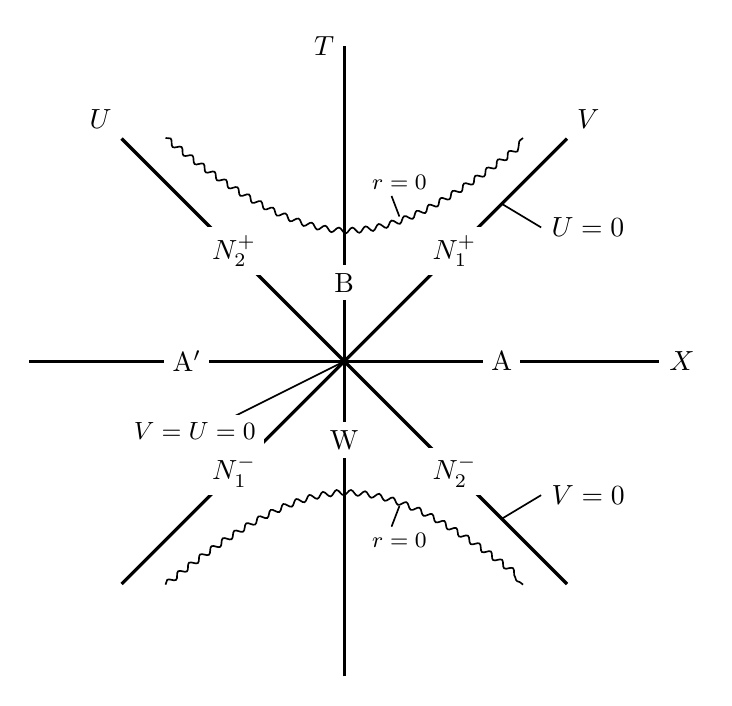
\begin{tikzpicture}[decoration={snake,segment length=5,amplitude=1}, semithick]
			\draw[\myarrow, very thick] (-4,0) -- (4,0);
			\draw[\myarrow, very thick] (0,-4) -- (0,4);
			\draw[\myarrow, very thick] (-2.828427,-2.828427) -- (2.828427, 2.828427);
			\draw[\myarrow, very thick] (2.828427, -2.828427) -- (-2.828427, 2.828427);
			% \draw[domain=-1:1,variable=\t] plot ({2*cosh(\t)},{2*sinh(\t)});
			\draw[domain=-1.1:1.1,variable=\t,decorate] plot ({1.7*sinh(\t)},{1.7*cosh(\t)});
			\draw[domain=-1.1:1.1,variable=\t,decorate] plot ({1.7*sinh(\t)},{-1.7*cosh(\t)});
			% \draw[domain=-1.3:1.3,variable=\t] plot ({1*sinh(\t)},{1*cosh(\t)});
			\node[right] (X) at (4, 0) {$X$};
			\node[left] (T) at (0, 4) {$T$};
			\node[above left] (U) at (-2.828427, 2.828427) {$U$};
			\node[above right] (V) at (2.828427, 2.828427) {$V$};
			\node (A) at (2,0) {\colorbox{white}{$\mathrm{A}$}};
			\node (Ap) at (-2, 0) {\colorbox{white}{$\mathrm{A'}$}};
			\node (B) at (0,1) {\colorbox{white}{$\mathrm{B}$}};
			\node (W) at (0, -1) {\colorbox{white}{$\mathrm{W}$}};
			\node (N1p) at (1.4, 1.4) {\colorbox{white}{$N_1^+$}};
			\node (N1m) at (-1.4, -1.4) {\colorbox{white}{$N_1^-$}};
			\node (N2p) at (-1.4, 1.4) {\colorbox{white}{$N_2^+$}};
			\node (N2m) at (1.4, -1.4) {\colorbox{white}{$N_2^-$}};
			\draw (2,2) -- (2.5,1.7);
			\node[right] (U0) at (2.4,1.7) {\colorbox{white}{$U=0$}};
			\draw (2,-2) -- (2.5,-1.7);
			\node[right] (V0) at (2.4,-1.7) {\colorbox{white}{$V=0$}};
			\draw (0,0) -- (-1.5, -0.75);
			\node[below] (UV0) at (-1.9, -0.55) {\colorbox{white}{\small $V=U=0$}};
			\draw (0.7, 1.83848) -- (0.6, 2.1);
			\node[above] (r1) at (0.7, 2.05) {\footnotesize $r=0$};
			\draw (0.7, -1.83848) -- (0.6, -2.1);
			\node[below] (r2) at (0.7, -2.05) {\footnotesize $r=0$};
		\end{tikzpicture}
		\caption{正文图 9-13(a)}
	\end{figure}
	\begin{zm}
		\begin{enumerate}[label = (\arabic*)]
			\item 对 $N_1$,
				\begin{align*}
					\tensorp{V}{^a} \Nabla{a} \tensorp{V}{^b} &= \frac{1}{4} \left( \tensorp{T}{^a} + \tensorp{X}{^a} \right) \Nabla{a} \left( \tensorp{T}{^b} + \tensorp{X}{^b} \right)\\
					&= \frac{1}{4} \left( \ChristoffelSymbol{\mu}{T}{T} + 2 \ChristoffelSymbol{\mu}{T}{X} + \ChristoffelSymbol{\mu}{X}{X} \right) \tensorp{x^\mu}{^b},
				\end{align*}
				显然 $x^\mu$ 只能取 $T$, $X$ 而不能取 $\theta, \phi$。易从 Kruskal 度规算得\footnote{如果懒得手搓,请参考第三章习题解答中的 Mathematica 代码}:
				\begin{align*}
					\ChristoffelSymbol{T}{T}{T} &= - \frac{r + 2M}{4Mr} \pdv{r}{T}, & \ChristoffelSymbol{T}{T}{X} &= - \frac{r + 2M}{4Mr} \pdv{r}{X}, & \ChristoffelSymbol{T}{X}{X} &= - \frac{r + 2M}{4Mr} \pdv{r}{T},\\
					\ChristoffelSymbol{X}{T}{T} &= - \frac{r + 2M}{4Mr} \pdv{r}{X}, & \ChristoffelSymbol{X}{T}{X} &= - \frac{r + 2M}{4Mr} \pdv{r}{T}, & \ChristoffelSymbol{X}{X}{X} &= - \frac{r + 2M}{4Mr} \pdv{r}{X},
				\end{align*}
				故
				\begin{align*}
					\tensorp{V}{^a} \Nabla{a} \tensorp{V}{^b} &= -\frac{r + 2M}{8Mr} \left( \pdv{r}{T} + \pdv{r}{X} \right) \left( \tensorp{T}{^b} + \tensorp{X}{^b} \right)\\
					&= - \frac{r + 2M}{4Mr} \left( \pdv{r}{T} + \pdv{r}{X} \right) \tensorp{V}{^a},
				\end{align*}
				而 $r = f(X^2 - T^2)$,故
				\begin{align*}
					\pdv{r}{T} + \pdv{r}{X} &= -2 T f' + 2X f' = - 2 U f'
				\end{align*}
				在 $N_1$ 上为零,故得证。同理可知 $U$ 是 $N_2$ 的仿射参数。

			\item 其余径向类光测地线在 Kruskal 坐标图示下也必须为倾斜 $\frac{\pi}{2}$ 的直线,即 $U$ 坐标线或 $V$ 坐标线。不妨考虑直线 $U = U_0$,其中 $U_0 \neq 0$,则以 $\lambda=r$ 为参数\footnote{这里多设一个参数 $\lambda$ 而不是直接写作 $r$ 是为避免测地线切矢的记号与 $r$ 坐标基矢引起混淆。},由于 $r = f(X^2 - T^2) = f(UV)$,其中 $f$ 的逆是
			\begin{equation*}
				f^{-1}(r) = \frac{r-2M}{2M} \e{r/2M},
			\end{equation*}
			则在测地线上有
			\begin{equation*}
				V = \frac{1}{U_0} f^{-1}(r),
			\end{equation*}
			切矢为
				\begin{align*}
					\tensorp{\lambda}{^a} &= \dv{V}{\lambda} \tensorp{V}{^a}\\
					&= \frac{r}{4M^2} \e{r/2M} \tensorp{V}{^a},
				\end{align*}
				故在曲线上,
				\begin{align*}
					\tensorp{\lambda}{^a} \Nabla{a} \tensorp{\lambda}{^b} &= \dv[2]{V}{\lambda} \tensorp{V}{^b} + \left( \dv{V}{\lambda} \right)^2 \tensorp{V}{^a} \Nabla{a} \tensorp{V}{^b}\\
					&= \left( \frac{r+2M}{8M^3} \e{r/2M} - \left( \dv{V}{\lambda} \right)^2 \frac{r+2M}{4Mr} \left( \pdv{r}{T} + \pdv{r}{X} \right) \right) \tensorp{V}{^b}\\
					&= \left( \frac{r+2M}{8M^3} \e{r/2M} - \left( \dv{V}{\lambda} \right)^2 \frac{r+2M}{2Mr} \dv{\lambda}{V} \right) \tensorp{V}{^b}\\
					&= \left( \frac{r+2M}{8M^3} \e{r/2M} - \dv{V}{\lambda} \frac{r+2M}{2Mr} \right) \tensorp{V}{^b}\\
					&= \left( \frac{r+2M}{8M^3} \e{r/2M} - \frac{r}{4M^2} \e{r/2M} \times \frac{r+2M}{2 Mr} \right) \tensorp{V}{^b}\\
					&= 0.
				\end{align*}
				若为测地线 $V = V_0$,同理可证。
		\end{enumerate}
	\end{zm}

	\item 引入与 Kruskal 坐标类似的坐标消除下列线元的坐标奇性 $r = R$:
	\begin{equation*}
		\dd s^2 = - \left( 1 - r^2/R^2 \right) \dd t^2 + \left( 1 - r^2/R^2 \right)^{-1} \dd{r}^2 + r^2 \left( \dd{\theta}^2 + \sin^2 \theta \dd{\phi}^2 \right) \qc R=\text{常数}.
	\end{equation*}
	\begin{jie}
		只考虑前两维,并取 $0<r<R$,
		\begin{equation*}
			\dd \hat{s}^2 = - \left( 1 - r^2/R^2 \right) \left( \dd t^2 + \left( 1 - r^2/R^2 \right)^{-2} \dd{r}^2 \right),
		\end{equation*}
		令
		\begin{equation*}
			r_* = \int_0^r \left( 1 - \frac{{r'}^2}{R^2} \right)^{-1} \dd{r'} = R \arctanh\left(\frac{r}{R}\right) \in (0, \infty),
		\end{equation*}
		则
		\begin{equation*}
			\dd{\hat{s}}^2 = \left( 1 - r^2/R^2 \right) \left( - \dd t^2 + \dd{r_*}^2 \right),
		\end{equation*}
		再令
		\begin{equation*}
			u := t - r_* \qc v := t + r_*,
		\end{equation*}
		其取值范围为
		\begin{equation*}
			v > u,
		\end{equation*}
		得
		\begin{equation*}
			\dd \hat{s}^2 = - \left( 1 - \frac{r^2}{R^2} \right) \dd{u} \dd{v},
		\end{equation*}
		令
		\begin{equation*}
			U := \e{-\beta u} \qc V := \e{\beta v},
		\end{equation*}
		其中 $\beta$ 是待定常数,则取值范围是
		\begin{equation*}
			U,V > 0 \qc UV > 1,
		\end{equation*}
		且
		\begin{align*}
			\dd \hat{s}^2 &= - \beta^{-2} \left( 1 - \frac{r^2}{R^2} \right) \e{\beta(u-v)} \dd{U}\dd{V}\\
			&= - \beta^{-2} \left( 1 - \frac{r^2}{R^2} \right) \left( \frac{R+r}{R-r} \right)^{-\beta R} \dd{U} \dd{V},
		\end{align*}
		若选择 $\beta = -1/R$,则
		\begin{align*}
			\dd \hat{s}^2 = - \left( R+r \right)^2 \dd{U} \dd{V},
		\end{align*}
		坐标奇性已被消除,只需将 $r$ 视作函数
		\begin{equation*}
			r = \frac{1 - U V}{1 + U V} R,
		\end{equation*}
		即可允许 $U, V$ 除 $U V = - 1$ 外任意取值,则 $U V > -1$ 定义了一个连通的延拓。还可进一步令
		\begin{equation*}
			T := \frac{1}{2} \left( V + U \right) \qc X := \frac{1}{2} \left( V - U \right),
		\end{equation*}
		则得到完整的延拓后度规
		\begin{equation*}
			\dd s^2 = \left( R + r \right)^2 \left( - \dd{T}^2 + \dd{X}^2 \right) + r^2 \left( \dd \theta^2 + \sin^2 \theta \dd \phi^2 \right),
		\end{equation*}
		其中
		\begin{equation*}
			r = \frac{1 - T^2 + X^2}{1 + T^2 - X^2} R.
		\end{equation*}
	\end{jie}

	\item 试证最大延拓施瓦西时空有 s.p. 曲率奇性。提示:利用式 (8-3-21)\footnote{正文(8-3-21)为
	\begin{equation}
		\left.
			\begin{gathered}
				\tensor{R}{_0_1_0_1} = -\frac{2M}{r^3} \qc \tensor{R}{_0_2_0_2} = \frac{M}{r} \left( 1 - 2M/r \right) \qc \tensor{R}{_0_3_0_3} = \frac{M}{r}\left( 1 - 2M/r \right) \sin^2\theta,\\
				\tensor{R}{_1_2_1_2} = - \frac{M}{r} \left( 1 - 2M/r \right)^{-1} \qc \tensor{R}{_1_3_1_3} = - \frac{M}{r} \left( 1 - 2M/r \right)^{-1} \sin^2 \theta \qc \tensor{R}{_2_3_2_3} = 2 M r \sin^2 \theta.
			\end{gathered}
		\right\}
		\tag{8-3-21}
	\end{equation}}。
	\begin{zm}
		由于 $B$ 区仍可使用施瓦西坐标,直接利用 (8-3-21) 得
		\begin{align*}
			\tensor{R}{^a^b^c^d} \tensor{R}{_a_b_c_d} &= \tensor{g}{^\mu^\alpha} \tensor{g}{^\nu^\beta} \tensor{g}{^\sigma^\gamma} \tensor{g}{^\rho^\delta} \tensor{R}{_\mu_\nu_\sigma_\rho} \tensor{R}{_\alpha_\beta_\gamma_\delta}\\
			&= \sum_{\mu,\nu,\sigma,\rho} \tensor{g}{^\mu^\mu} \tensor{g}{^\nu^\nu} \tensor{g}{^\sigma^\sigma} \tensor{g}{^\rho^\rho} \left( \tensor{R}{_\mu_\nu_\sigma_\rho} \right)^2\\
			&= \frac{4M^2}{r^6} + \frac{M^2}{r^6} + \frac{M^2}{r^6} + \frac{M^2}{r^6} + \frac{M^2}{r^6} + \frac{4M^2}{r^6}\\
			&= \frac{12 M}{r^6},
		\end{align*}
		故当不完备测地线(例如题8.8中以 $r$ 为仿射参数的径向类光测地线)趋于 $r=0$ 时,具有 s.p. 曲率奇性。
	\end{zm}

	\item 试证图 9-13(a) 的 $N_1$ 是类光超曲面。提示:只须证明其法矢 $\tensor{n}{^a}$ 类光。请注意 $N_1$ 的方程为 $U=0$,其法余矢为 $\tensor{n}{_a} = \Nabla{a} U$。
	\begin{zm}
		\begin{align*}
			\tensor{g}{^a^b} \tensor{n}{_a} \tensor{n}{_b} &= \tensor{g}{^a^b} \tensord{U}{_a} \tensord{U}{_b}\\
			&= \tensor{g}{^U^U}\\
			&= 0,
		\end{align*}
		其中 $\tensor{g}{^U^U}$ 指 $\tensor{g}{^a^b}$ 在 $\{ U, V, \theta, \phi \}$ 坐标系中的 $UU$ 分量。
	\end{zm}
\end{xiti}
